\documentclass[10pt,twocolumn,letterpaper]{article}
% PACKAGES ===================================================================================
\usepackage{iccv}
\usepackage{times}
\usepackage{epsfig}
\usepackage{graphicx}
\usepackage{color}
\usepackage{amsmath,amssymb}
\usepackage{algorithm,algpseudocode}
\usepackage{subfig}
\graphicspath{{./figures/}}
\DeclareGraphicsExtensions{.pdf,.jpeg,.png,.jpg}

% Include other packages here, before hyperref.

% If you comment hyperref and then uncomment it, you should delete
% egpaper.aux before re-running latex.  (Or just hit 'q' on the first latex
% run, let it finish, and you should be clear).
\usepackage[pagebackref=true,breaklinks=true,letterpaper=true,colorlinks,bookmarks=false]{hyperref}

% ============================================================================================
% COMMENTS
% ============================================================================================
\newcommand{\stavros}[1]{{\textcolor{red}{[\emph{stavros}: #1]}}}

% ============================================================================================
% GENERAL DEFINITIONS
% ============================================================================================
\usepackage{xspace}
\def\sota{state-of-the-art}
\def\groundtruth{ground truth}
\def\CUB{CUB-200-2011}
\def\eg{\emph{e.g}\onedot} \def\Eg{\emph{E.g}\onedot}
\def\ie{\emph{i.e}\onedot} \def\Ie{\emph{I.e}\onedot}
\def\cf{\emph{c.f}\onedot} \def\Cf{\emph{C.f}\onedot}
\def\etc{\emph{etc}\onedot} \def\vs{\emph{vs}\onedot}
\def\wrt{w.r.t\onedot} \def\dof{d.o.f\onedot}
\def\etal{\emph{et al}\onedot}
\def\kmeans{\emph{k}-means}
\def\cpp{C\texttt{++}}
\def\matlab{MATLAB}
\def\matconvnet{MatConvNet}

% Chapters, Sections, Figures, Equations
\newcommand{\refchap}[1]{Chapter~\ref{#1}}
\newcommand{\refsec}[1]{Section~\ref{#1}}
\newcommand{\reffig}[1]{Figure~\ref{#1}}
\newcommand{\refeq}[1]{Equation~\ref{#1}}
\newcommand{\refalg}[1]{Algorithm~\ref{#1}}
\newcommand{\reftab}[1]{Table~\ref{#1}}
\newcommand{\refapp}[1]{Appendix~\ref{#1}}

% ============================================================================================
% MATH DEFINITIONS 
% ============================================================================================
\newcommand{\pd}[2]{\frac{\partial #1}{\partial #2}}
\newcommand{\mat}[1]{\mathbf{#1}} 
\renewcommand{\vec}[1]{\mathbf{#1}}
\newcommand{\set}[1]{\mathcal{#1}}
\newcommand{\inprod}[1]{{\left< \, #1 \, \right>}}
\newcommand{\R}{\mathbb{R}}
\def\abs{\operatorname{abs}}
\DeclareMathOperator*{\argmin}{arg\,min}
\DeclareMathOperator*{\argmax}{arg\,max}
\newcommand{\p}[1]{\vec{p}_{#1}} 	 % point in space domain with subscript
\newcommand{\f}[1]{\vec{f}_{#1}} 	 % point in space domain with subscript
\newcommand{\g}[1]{\vec{g}_{#1}} 	 % point in space domain with subscript
\newcommand{\norm}[1]{\left \lVert #1 \right \rVert} % norm
%\newcommand{\norm}[1]{|| #1 ||} % norm


% \iccvfinalcopy % *** Uncomment this line for the final submission

\def\iccvPaperID{****} % *** Enter the ICCV Paper ID here
\def\httilde{\mbox{\tt\raisebox{-.5ex}{\symbol{126}}}}

\begin{document}
\title{AMAT: Computing the Medial Axis Tranform for Natural Images Using a Weighted Geometric Set Cover Approach}
\maketitle
%\thispagestyle{empty}


%%%%%%%%% ABSTRACT
\begin{abstract}
The medial axis transform (MAT) is a powerful shape abstraction that has been successfully
used in shape summarization, matching and retrieval. 
Despite the MAT's long history, the lack of an adequate definition and evaluation criterion 
that can accommodate color and texture have prevented its widespread use for tasks involving natural images.
In this paper we propose a new formulation of the
MAT for natural images as a weighted geometric set cover (WGSC) problem, and we use a greedy 
approximation algorithm to solve it.
Our method, called Appearance-MAT (AMAT), makes the following contributions: 
i) it extends previous methods for color images, which were limited to only returning medial point locations, 
by associating  each medial point with a local scale; 
ii) inspired by the invertibility property of the 
original MAT for binary images, it also associates each medial point with a local encoding
which allows us to invert the AMAT, faithfully reconstructing the input image; 
iii) this additional information enables grouping individual points into medial branches,
which correspond to meaningful image regions, supporting both image segmentation and boundary
ownership assignment.
We perform experiments in medial point detection on a new dataset of medial axes, called
Berkeley-Medial AXes (BMAX500), based on the popular BSDS500 dataset.
We also measure the quality of the reconstructed images from the same dataset,
obtained by inverting their computed AMAT. 
Finally, we show that edge maps extracted as a by-product of our method
can be integrated in popular object proposal pipelines, thereby boosting performance.
Our code will be made publicly available.
\end{abstract}



%%%%%%%%% BODY TEXT %%%%%%%%%%%%%%%%%%%%%%%%%%%%%%%%%%
% ====================================================================================================================
\section{Introduction}\label{sec:introduction}
% ====================================================================================================================
\begin{figure}[!t]
\centering
\subfloat[Input image]{\includegraphics[width=0.47\linewidth]{teaser_img.pdf}\label{fig:teaser:input}}
\subfloat[Binary MAT]{\includegraphics[width=0.47\linewidth]{teaser_mat.pdf}\label{fig:teaser:mat}} \\
\subfloat[Appearance-MAT]{\includegraphics[width=0.47\linewidth]{teaser_amat.pdf}\label{fig:teaser:amat}}
\subfloat[Reconstructed image]{\includegraphics[width=0.47\linewidth]{teaser_recon.pdf}\label{fig:teaser:recon}}
\caption{\textbf{Top:} Input image (\ref{fig:teaser:input}) and segmentation (\ref{fig:teaser:mat}) from BSDS500,
using a different color for each ground-truth segment. 
We overlay ground-truth medial axes extracted from each segment using~\cite{telea2002augmented} (green) and a subset of medial disks (red). 
Using the medial disk radius information, we can reconstruct the input segments. 
\textbf{Bottom:} Similarly, the Appearance-MAT (\ref{fig:teaser:amat}) carries enough information to reconstruct the 
 \emph{input image} (\ref{fig:teaser:recon}) with just $\sim 5\%$ of the pixels 
 (we use white color for non-medial points in~\ref{fig:teaser:amat}).}
\label{fig:teaser}
\end{figure}


Symmetry is a ubiquitous property in the natural world, with a well-established role in human vision.
Humans instinctively recognize and use symmetry to analyze complex scenes, as it facilitates the encoding of shapes and
their discrimination and recall from memory~\cite{barlow1979versatility,royer1981detection,wagemans1998parallel}.
\stavros{check references for importance of symmetry in human vision in the scale axis transform paper}
In the context of computer vision, \emph{local} symmetry is of particular interest, 
because of its robustness to viewpoint changes and its connection to salient structures, such as object parts.
This intuition is fundamental in many milestones in object representation theory, including generalized
cylinders~\cite{binford1971visual}, superquadrics~\cite{barr1981superquadrics}, 
geons~\cite{biederman1987recognition}, and shock graphs~\cite{siddiqi1999shock}.

Fundamental notions of local symmetry were introduced decades ago by Blum in the context 
of binary shapes~\cite{blum1967transformation,blum1973biological} with the \emph{medial axis transform (MAT)}.
The MAT is a powerful abstraction of 2D and 3D shapes 
that has been successfully used in shape recognition, matching and retrieval. 
One of its most important strengths is that it provides a very compact representation that can
be used to accurately reconstruct the input shape. 
This makes the MAT very useful for reducing the complexity and computational demands for various algorithms.
As a result, many researchers have focused their efforts on achieving a good balance
between MAT sparsity and the reconstruction quality~\cite{tam2003shape,li2015q}.

Despite the MAT's long history, the lack of a definition and evaluation criterion 
that accommodates color and texture have prevented its widespread use for tasks involving natural images.
Previous works have mostly attacked the sub-problem of \emph{medial point detection}~\cite{tsogkas2012learning,shen2016object}.
Solving this problem amounts to determining the \emph{locations} of medial points (points lying on the medial axis) 
but not the scale of the respective medial disk.
The type of medial axes considered is also constrained to make the problem more concrete.
\cite{tsogkas2012learning} only considers medial axes of elongated structures, while~\cite{shen2016object} 
focuses on detecting \emph{object} skeletons, ignoring background structures.
These methods also lack another key characteristic of the MAT: medial point locations alone do not provide sufficient
information to reconstruct the input.

In this paper we introduce the first ``complete'' MAT for natural images, dubbed \emph{Appearance-MAT (AMAT)}.
First, we provide a new MAT definition in the context of natural images by framing it 
as a weighted geometric set cover (WGSC) problem.
Our definition is centered around the invertibility property of the binary MAT, and elicits 
a straightforward criterion for quality assessment, in terms of input image reconstructions obtained by inverting their AMAT.
Second, our algorithm associates each medial point with \emph{scale} as well as local \emph{appearance} information
that can be used to faithfully reconstruct the input.
Thus, the AMAT encompasses all the fundamental features of its  binary counterpart. 
Third, we describe a simple bottom-up grouping scheme that exploits the additional scale and appearance information to connect
points into medial \emph{branches}.
These branches correspond to meaningful image regions, and extracting them can support both image segmentation
and boundary ownership assignment.
Finally, being bottom-up in nature, our method does not assume any object-level knowledge.
It computes medial axes of foreground and background structures equally, 
and results in a compact representation that only uses $5-10\%$ of the pixels in the original image.
This sparse set of points carries enough information to reconstruct the input, therefore it
can replace the original image in algorithms for tasks such as scene classification 
or image retrieval, significantly reducing their running time.

We perform experiments in medial point detection on a new dataset of medial axes, the 
\emph{Berkeley-Medial AXes (BMAX500)}, which is built on the popular BSDS500 dataset, showing \sota\ performance.
We also measure the quality of reconstructions  obtained by inverting the AMAT of images from the same dataset, 
using  a variety of standard image quality metrics.
We compare with two reconstruction baselines: one built on the medial point detection algorithm from~\cite{tsogkas2012learning}
and one built from the ground-truth segmentations in BSDS500.
Our methods outperforms the baselines in terms of reconstruction quality, while attaining a better compression and
compression-to-quality ratio.

The outline of the paper is as follows: we start by reviewing related work on medial axis extraction for binary shapes
and natural images in~\refsec{sec:related}.
In~\refsec{sec:method} we describe our approach; we define the problem, introduce notation, and highlight the connection to
the WGSC problem.
We also discuss the schemes for bottom-up grouping of the medial points into branches and the AMAT simplification.
~\refsec{sec:implementation} includes implementation details and in~\refsec{sec:experiments} we present our results.
Finally, in~\refsec{sec:discussion} we conclude and discuss ideas for future directions.


% ====================================================================================================================
\section{Related Work}\label{sec:related}
% ====================================================================================================================
\subsection{MAT for binary shapes}\label{sec:related:binary}
Blum introduced the concept of the medial axis transform, or skeleton, for two-dimensional shapes,
in  his seminal works~\cite{blum1967transformation,blum1973biological}.
Since then, many other researchers have developed algorithms for more reliable
and more efficient medial axis extraction, its extension to 3D shapes, and its application
to computer vision tasks.

Siddiqi~\etal define \emph{shocks} as the singularities of a curve evolution process acting on the boundaries of
a shape, and they organize them into a directed, acyclic shock graph~\cite{siddiqi1999shock}.
Shock graphs were successfully used in shape matching~\cite{siddiqi1999shock}, recognition~\cite{sebastian2001recognition},
and database indexing~\cite{sebastian2002shock}.
\emph{Bone graphs}~\cite{macrini2008skeletons} offer improved stability and a more intuitive representation of an object's parts, 
compared to skeletons and shock graphs, by identifying and analyzing ligature structures.
Visual part correspondences are also established and used to measure part and aggregated shape similarity in~\cite{latecki2000shape}.
The idea of object parts corresponding to endpoints of skeleton branches is further explored in~\cite{bai2008path}, where
\emph{geodesic} paths between skeleton endpoints are used to match the respective graphs.
More recently, Stolpner \etal deal with the problem of approximating a 3D solid via a union
of overlapping spheres~\cite{stolpner2012medial}.

The value of the MAT has been equally (if not more) appreciated by the graphics community, where object shapes 
are routinely represented as point clouds or triangular meshes.
Giesen~\etal~\cite{giesen2009scale} introduced the \emph{scale axis transform}, a skeletal shape representation
that yields a hierarchy of successively simplified skeletons, which are obtained by multiplicative scaling of the
MAT's radii.
Li~\etal~\cite{li2015q} use quadratic error minimization to compute an accurate linear approximation of the MAT, called \emph{Q-MAT}.
They show experiments on medial axis simplification where they reduce the number of nodes of an initial medial mesh
by three orders of magnitude, while preserving good surface reconstruction.


\subsection{MAT for natural images}\label{sec:related:natural}
Compared to the binary setting, the number of works on medial axis detection for natural images is rather limited.
Levinstein \etal~\cite{levinshtein2009multiscale} attack the problem of detecting \emph{symmetric parts} in objects
by learning to merge adjacent deformable maximal inscribed disks, modeled as superpixels.
Learned non-accidental part attachment relations are then used to combine proximal detected parts into coarse skeletal representations.
Lee \etal extend that work by introducing a deformable disk model that can capture curved and tapered parts, and also add
continuity constraints to the medial point grouping process~\cite{lee2013detecting}.
In other works medial point detection is posed as a classification problem where the goal is to label image pixels
as ``medial'' or ``not-medial'', inspired by similar methods for boundary detection~\cite{martin2004learning,arbelaez2011contour}.
Tsogkas and Kokkinos use a multiple instance learning (MIL) framework to deal with the unknown scale and orientation 
during training~\cite{tsogkas2012learning}, while, more recently, Shen \etal adapt a deep CNN with 
side outputs~\cite{xie2015holistically} for the task of extracting \emph{object skeletons}~\cite{shen2016object}.
All these approaches exploit appearance information by incorporating some sort of machine learning algorithm.

Our work can be regarded as lying at the intersection of previous work on binary and natural images.
From a technical standpoint, it shares more similarities with binary methods, for instance~\cite{stolpner2012medial},
which solves the set cover problem for volumes in the 3D space.
At the same time, it can be applied to real images, without assuming a figure-ground segmentation,
but it also demonstrates unique characteristics.
Our method does not involve learning, and is not constrained in detecting a particular subset of
medial axes as~\cite{tsogkas2012learning,shen2016object}.
It also complements existing methods by augmenting point locations with scale and appearance descriptions, which
are necessary for reconstructing the input.


% ====================================================================================================================
\section{Method}\label{sec:method}
% ===================================================================================================================
\subsection{Problem Definition}\label{sec:method:definition}
Consider a 2D binary shape, $O$, in the image plane, and its boundary $\Theta_O$.
The \emph{medial axis} of $O$ is the set of points $\p{}$ that lie midway between two sections of 
its boundary. The points $\p{}$ are the centers of maximally inscribed (medial) disks, bitangent to $\Theta_O$
in the interior of the shape. The disk radius $r(\p{})$ is the distance between $\p{}$ and 
the points where the disk touches $\Theta_O$, and is called the \emph{medial radius}.
The process of mapping $O$ to the set of point-radius pairs $(\p{},r(\p{})) \in \mathbb{R}^2 \times \mathbb{R}$
is called the \emph{medial axis transform} (MAT).
Given these pairs, we can reconstruct the object as a union of overlapping disks that sweep-out 
its interior by ``expanding'' a value of one (1) inside the area covered by each  medial disk.

We argue that a MAT for real images should satisfy a similar principle: given the MAT of an image, 
we should be able to ``invert'' it, reconstructing \emph{the image} itself.
There are several reasons why extending this idea to real images is a challenging task. 
Natural images contain complex scenes and are cluttered with various objects, instead of a single foreground shape.
Moreover, whereas binary images are composed of uniform areas of zeros (0) and ones (1), 
real images obey complicated color and texture distributions.
Nevertheless, we can exploit image redundancies and assume that an image is composed of many small regions of 
relatively uniform appearance.
This is a concept on which most superpixel algorithms rely on for breaking up an image 
into non-overlapping patches, while respecting perceptually meaningful region 
boundaries~\cite{shi2000normalized,levinshtein2009turbopixels,achanta2012slic}. 

\paragraph{Notation:} Before proceeding with our formulation, we list the notation used throughout the paper.
We use capital italics for single elements and capital calligraphic letters to denote sets. A disk of radius $r$,
centered at point $\p{}$ is denoted as $D(\p{},r)=D_{\p{},r}$. 
For brevity, we ofter refer to such a disk as a $r$-disk or $(\p{},r)$-disk.
We will also occasionally use $r(\p{}) = r_{\p{}}$ to refer to the radius/scale $r$, associated with point $\p{}$.
$\set{D}$ is a collection of such disks of varying centers and radii, $\set{D}=\{ D_{\p{i},r_{\p{i}}} \},\, i\in\mathbb{N}$.
The interesection of a $(\p{},r)$-disk with an image $I$ is a disk-shaped region of the image, and is denoted by 
$I \cap D_{\p{},r}=D_{\p{},r}^I \subset I$. Finally, we use $\circ$ to denote function composition.

\paragraph{Formulation:} Consider an RGB image $I\subset\R^2$, and a disk-shaped region $D_{\p{},r}^I \subset I$.
Let $f:\R^2 \rightarrow \R^K$ be a function that maps $D_{\p{},r}^I$ to a vector representation $\f{\p{},r}=f\circ D_{\p{},r}^I$. 
We call this vector the \emph{encoding} of $D_{\p{},r}^I$. 
Now let $g:\R^K \rightarrow \R^2$ be a function that maps $\f{\p{},r}$ back to a disk patch $\tilde{D}_{\p{},r}^I$: 
$\g{\p{},r} = g \circ \f{\p{},r} = \tilde{D}_{\p{},r}^I$. We call $g$ the \emph{decoding} function.
In the general case, $f$ and $g$ will be \emph{lossy} mappings, which means that the reconstruction error 
$e_{\p{},r} = \norm{ \tilde{D}_{\p{},r}^I - D_{\p{},r}^I}_2^2 \geq 0$. 
Using the above notions, we define the MAT as the set of tuples 
$M:\{ ( \p{1},r_{\p{1}}, \f{\p{1},r_{\p{1}}}, \ldots, ( \p{m},r_{\p{m}}, \f{\p{m},r_{\p{m}}} ) \}$, such that:
\begin{equation}
M = \argmin_{\p{},r}{\sum_{i=1}^m e_{\p{i},r_i}},\quad I=\bigcup_{i=1}^m D_{\p{i},r_i}^I 
\label{eq:minimization}
\end{equation}
\paragraph{Encoding and decoding functions:}
Our framework allows $f,g$ to take any form; 
for example, $f$ could be a histogram representation of color in $D_{\p{},r}^I$ and $g$ could return the mode of the distribution.
In this paper we opt for simplicity:
$f$ computes the mean of each color channel ``summarizing'' $D_{\p{},r}^I$, in a $3\times1$ vector $\f{\p{},r}$.
Conversely, $g$ constructs an approximation $\tilde{D}_{\p{},r}^I \approx D_{\p{},r}^I$ by replicating $\f{\p{},r}$ in the
respective disk-shaped area.
When the $(\p{},r)$-disk is fully enclosed in a region with uniform color, the reconstruction error $e_{\p{},r}$
is low, whereas when the disk crosses a strong image boundary, the encoding $\f{\p{},r}$ cannot accurately represent
the underlying image region, resulting in a higher error. 
Because we augment each point by adding local appearance information in the form of $\f{\p{},r}$, 
we dub our approach \emph{Appearance}-MAT or \emph{AMAT}.

Note that the definition in~\refeq{eq:minimization} suggests conceptual similarities with superpixel representations.
Selecting the points $\{ (\p{i},r_i,\f{\p{i},r_i}) \},\,i=1,\ldots,m$ is equivalent to covering the input image
with $m$ disk-shaped superpixels. Minimizing the total reconstruction error implies that these ``superdisks'' do not
cross region boundaries, as this would incur a high reconstruction error, as shown in~\reffig{fig:google}.
However, there are two important differences:
First, in our case a canonical shape (disks) is used, whereas superpixels can have any form. 
Second, our disks are \emph{overlapping}, in contrast to standard, non-overlapping superpixels.

\begin{figure}[ht]
\centering
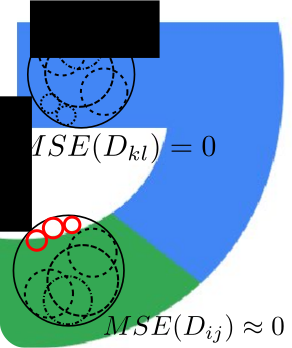
\includegraphics[width=\linewidth]{google_disks.pdf}
\caption{$\mathbf{D_W:}$ Composing an image using overlapping disks; disk centers form the medial axis (green points).
$\mathbf{D_G}$ lies at the intersection of three regions, so its encoding cannot accurately reconstruct the local image patch.
$\mathbf{D_R}$ incurs a small MSE, even though it does not respect region boundaries.
Comparing a disk's encoding $\f{B}$ to the encodings $\f{i}$ of \emph{all} contained disks provides a more robust
error metric.
}
\label{fig:google}
\end{figure}

\subsection{AMAT as a Geometric Set Cover Problem}\label{sec:method:wgsc}
The geometric set cover is the extension of the well studied set cover problem, in a geometric space.
For simplicity, here we only consider the case of a two-dimensional space and we particularly focus in the 
\emph{weighted} version of the problem, which is defined as follows:
Consider a universe of $n$ points $\set{X} \in \R^2$ and a family of sets 
$\set{D} = \{D_1,D_2,\ldots,D_m\} \subseteq \set{X}$. 
A common choice for these sets are intersections of $\set{X}$ with simple shape primitives, such as disks or rectangles.

Now assume that each set in $\set{D}$ is associated with a non-negative weight or \emph{cost} $c_i$.
Solving the WGSC problem amounts to finding a sub-collection $\bar{\set{D}} \in \set{D}$ that covers the entire $\set{X}$
(all $N$ elements of $\set{X}$ are contained in at least one set in $\bar{\set{D}}$), while having the minimum
total cost $C$; the total cost is simply the sum of costs of individual elements in $\bar{\set{D}}$.
WGSC is a strongly NP-hard problem for which polynomial-time approximate solutions (PTAS) exist.
Perhaps the simplest and most straightforward is the greedy algorithm described in~\cite{vazirani2013approximation}. 
The interested reader can find more details on WGSC and related algorithms 
in~\cite{mustafa2015quasi,varadarajan2010weighted,har2012weighted,chan2012weighted}.

The AMAT formulation described in~\refsec{sec:method:definition} lends itself naturally to a 
WGSC interpretation.
The input image $I\subset\R^2$ is the universe of $N$ points.
For practical reasons, we only consider $r$-disks with $r$ chosen from a finite set of radii $\set{R}:\{r_1,r_2,\ldots,r_R\}$.
The $r$-disks, $r\in\set{R}$ can be placed at any position $\p{}=(x,y)\in I$ such that $D_{\p{},r}$ is fully contained in $I$.
We also assign a cost $c_{\p{i},r_j} = c_{ij}$ to each possible $(\p{i},r_j)$-disk, $i\in[1,N],\, j\in[1,R]$.
This cost is directly related to the reconstruction cost 
$e_{\p{i},r_j} = e_{ij}$, given the functions $f,g$.
Note that for brevity, we drop the subscripts $\p{i},r_j$ and simply use $ij$ to refer to a $(\p{i},r_j)$-disk.
We provide more details regarding computation of $e_{ij}$ in~\refsec{sec:implementation}.

As~\refeq{eq:minimization} suggests, the goal is to find a subset of disks that cover the entire image, while maintaining
a low total reconstruction cost. 
A trivial solution would be to select each pixel as a disk of radius $r=1$, in which case
$M:\{ (\p{1},r_{\p{1}},f_{\p{1},r_{\p{1}}}), \ldots, ( \p{N},r_{\p{N}},f_{\p{N},r_{\p{N}}} ) \}$,
and $\sum_{i=1}^N e_{\p{i},r_i} = 0$; each pixel can be perfectly represented by its mean value.
Such a solution is of no practical usefulness. 
Staying true to the spirit of the medial axis transform, we seek a solution that is \emph{sparse}
(low number of medial points $m$), while being able to adequately reconstruct the input image.
One possible way to do this would be to agree on a fixed ``budget'' of points, and look for the 
optimal solution given $m$.
However choosing an acceptable $m$ can be a nuisance, as its value can vary significantly  from image to image.

In the original MAT, sparsity is implicitly induced through the use of maximal disks,
touching the shape boundary at exactly two points.
Extending the maximality principle to the case of natural images is not straightforward,
as the notion of color and texture boundaries is not robustly defined.
Relying on the output of a boundary extraction algorithm is not an option either,
as it would make our method very sensitive to errors from which it would be impossible to recover.
We choose to regularize the minimization criterion in~\refeq{eq:minimization} in an alternative way. 
We add a scale-dependent term $s_j = \frac{w_s}{r_j}$ to the costs $c_{ij}$, with $s_j$ 
being inversely proportional to the radius $r_j$.
This way we favor the selection of larger disks at each point, as long as $s_j$ is not ``too'' large
with respect to the error incurred by picking $D_{\p{},r_{j+1}}$ instead of $D_{\p{},r_j}$.
Selecting a high value for $w_s$ will lead to a sparser solution with higher total reconstruction error $E$,
whereas a low value for $w_s$ will aim for a higher reconstruction quality, by utilizing more, smaller disks
to cover $I$.

\paragraph{Greedy approximation algorithm:}
There are many polynomial-time-approximate-solution (PTAS) algorithms for the vanilla set cover
and its geometric variants.
Since this is the first attempt on applying a WGSC approach to compute the MAT of real images, we keep things simple
and use the greedy algorithm described in~\cite{vazirani2013approximation}, adapted for the weighted case.
The steps of our method are described in~\refalg{alg:greedy}
\begin{algorithm}[t]
\caption{AMAT greedy algorithm.}
\label{alg:greedy}
	\begin{algorithmic}[1]
	\Statex \textbf{Input:} $X,I=\{\p{1},\ldots,\p{N}\},\set{R}=\{r_1,\ldots,r_R\},f,g$.
	\Statex \textbf{Output:} $M$
	\State Initialization: $M \leftarrow \emptyset,X \leftarrow \emptyset$.
	\State Compute $f_{\p{},r},\, g_{\p{},r} = g \circ f_{\p{},r},\,\, \forall \p{} \in I, \forall r \in \set{R}$.
	\While{$X \subset I$}
		\State $c_{\p{},r}^e = \frac{c_{\p{},r}}{|D_{\p{},r} \setminus X|}+\frac{w_s}{r},\,\, \forall \p{} \in I, \forall r \in \set{R}$.
		\State $(\p{}^{*},r^{*}) = \argmin_{\p{},r}{c_{\p{},r}^e}$.		
		\State $M\leftarrow M\cup{(\p{}^{*},r^{*},f_{\p{}^{*},r^{*}})}$.
		\State $X \leftarrow X\cup D_{\p{}^{*},r^{*}}$ 
	\EndWhile
	\end{algorithmic}
\end{algorithm}
We start by computing the costs $c_{ij}$ for all possible disks $D_{ij}$.
We define the \emph{effective cost} of $D_{ij}$ as $c_{ij}^e = \frac{c_{ij}}{A_{ij}} + s_j$ , where $A_{ij}$ is the number
of \emph{new} pixels covered by $D_{ij}$ (pixels that have not been covered by a previously selected disk).
Starting from an empty set $M$, we pick the disk with the lowest $c_{ij}^e$ and add it to the solution, 
removing the area $D_{ij}$ from the pixels that have to be covered.
This process is repeated until all image pixels have been covered by at least one disk.

\subsection{Grouping Medial Points Into Branches}\label{sec:method:grouping}
The scale and appearance associated with each medial point provide a useful
description that can be used to group points belonging in the same region into \emph{medial branches}.
The beneficial effects of grouping in low-level vision tasks have been
observed in previous works~\cite{felzenszwalb2006min,zhu2007untangling,kokkinos2010highly,qi2015making}.
In our case, grouping pixels into branches can help us both refine the final medial axis, 
by aggregating consensus from neighboring points, and reduce complexity 
by allowing us to manipulate sets of points jointly.

We group detected medial points using an agglomerative scheme that starts at fine scales and
progressively merges together nearby points at coarser scales.
Our grouping criterion relies in proximity in \emph{scale-space} and \emph{appearance}.
Intuitively, points that are very close in the image, have higher probability of belonging in the
same contour.
We also expect that the scale of neighboring points on the same curve will change \emph{gradually}.
so points that lie close to one another but have very different scales should probably not be grouped together.
Finally, two points should not be merged if their encoding appearance vectors are very dissimilar,
as this indicates that they belong to different regions, regardless of their proximity in scale-space.

We combine these ideas into the clustering scheme described in~\refalg{alg:grouping}.
We initialize branches as the connected components of the AMAT output.
Starting at a scale $r_j$, we consider one branch at a time, and examine all other
branches within a neighborhood of size $r_j \times r_j$ and a scale neighborhood $[r_{j-3},r_j]$.
If two branches coexist in this scale-space neighborhood and their average encodings are similar,
they are merged.
The grouping algorithm terminates when all scales have been considered.

\begin{algorithm}[t]
\caption{Point grouping algorithm.}
\label{alg:grouping}
	\begin{algorithmic}[1]
	\Statex \textbf{Input:} $\set{R}=\{ r_1,\ldots.r_R \}, \newline M=\{ (\p{i},r_{\p{i}},\mathbf{f}_{\p{i},r_{\p{i}}}) \}, \, i=\in[1,m]$.
	\Statex \textbf{Output:} $B= \{ \mathbf{b}_1,\ldots,\mathbf{b}_k \} = \newline \{ (\p{l_{11}},\ldots,\p{l_{1i}}), \ldots, (\p{l_{k1}},\ldots,\p{l_{kj}}) \},\, l_{ij}\in[1,m]$.
	\State Initialization: $B \leftarrow cc(M)$. \Comment{Connected components}
	\ForAll{scales $r_i$}
		\ForAll{branches $\mathbf{b}_j$}
		\EndFor
	\EndFor
	\end{algorithmic}
\end{algorithm}
\stavros{Complete and keep the grouping pseudocode only if space permits}


\subsection{Medial Branch Simplification}\label{sec:method:simplification}
The output of our algorithm captures mostly region centerlines but there are still
imperfections in the form of noisy responses or ``lumps'', instead of thin contours.
Such imperfections are expected since the greedy algorithm provides only an approximate solution
to the minimization problem of~\refeq{eq:minimization}. 
In addition, because we use a discrete grid, the placement of disks 
in the image domain does not always result in their centers spanning a continuous curve, 
which leads to isolated medial points.

Grouping MAT points into branches makes it possible to process each branch individually, enabling
the correction of these errors post hoc.
We perform simple morphological operations (dilation and thinning) 
on the points of each branch to merge neighboring and isolated pixels together, while removing 
redundant responses. 
We also adjust the scales of the medial points after thinning, to ensure that the medial disks corresponding 
to the simplified structure span the same image area.
Because grouped branches correspond to relatively homogeneous regions, we expect that reconstruction
results after simplification will not change much.
Examples of simplified medial axes are illustrated in~\reffig{fig:experiments:detection:examples}.
With a negligible drop in reconstruction quality, we are able to achieve a dramatic reduction
in the number of medial points, and produce much cleaner medial axes.


% =============================================================================================
\section{Implementation Details}\label{sec:implementation}
% =============================================================================================
\subsection{Disk Cost Computation}\label{sec:implementation:diskcost}
The greedy algorithm described in~\refsec{sec:method:wgsc} requires assigning a cost to all possible disks $D_{ij}$.
Choosing an appropriate type of cost function is crucial towards obtaining a final MAT that both incorporates
the use of maximal disks, leading to a sparse solution, and faithfully reproduces the input image.
Since our objective is high reconstruction quality, $c_{ij}$ should be directly proportional
to the reconstruction error of the local image patch.
Given our choice of functions $f,g$, using a criterion such as MSE or PSNR will not work.
These metrics are well known to perform poorly in representing perceptual similarity of images~\cite{girod1993what,wang2009mean}.
For example, \reffig{fig:google} shows that naively selecting a disk with a low MSE score does not guarantee that it 
respects image boundaries.
Instead, we would rather select disks whose encodings are representative of \emph{all} disks that are fully enclosed
in their area. 

First, we convert the RGB input image to the CIELAB color space which is more suitable for measuring perceptual distances,
and perform all our computations in that space.
We define the cost for a disk $D_{\p{i},r_j}$ as follows:
\begin{equation}
c_{ij} = \sum_k \sum_l \norm{\mathbf{f}_{ij} - \mathbf{f}_{kl} }^2 \quad \forall k,l: D_{kl} \subset D_{ij}
\label{eq:diskcost}
\end{equation}
Intuitively, a low cost $c_{ij}$ implies that the encoding $\mathbf{f}_{ij}$ is representative of \emph{all}
the disks that are fully contained in $D_{ij}$, hence $D_{ij}$ is not crossing any region boundaries.

Computing $c_{ij}$ can be very demanding as it requires to compute encoding differences for all 
disks in $D_{ij}$; if $r_j$ is large, this number can grow very quickly.
We can significantly reduce computation time by i) using convolutions to compute the sums in~\refeq{eq:diskcost}
and ii) minimizing redundant computations by using cumulative sums over \emph{circular} areas instead of disks.
An alternative way to speedup performance is using rectangular or square shapes as the
shape elements we use to cover the image domain.
Using square filters would allow us to compute sums within regions with a fixed number of operations per position on an integral
image~\cite{viola2001rapid,arbelaez2011contour}, reducing complexity by an order of magnitude.
We leave this as a future extension and include further details for our current implementation in the supplemental material.


\subsection{Dealing with textured images}\label{sec:implementation:texture}
The main motivation behind the choice of simple functions $f,g$, such as the ones described in~\refsec{sec:method:definition}, was simplicity and 
computational efficiency.
Such functions also allow us to inject certain desired characteristics to the regions depicted by medial points in the AMAT solution.
for instance, appearance uniformity and alignment with boundaries.
However, natural images often contain high-frequency textures or noise and noise, which can lead to the accumulation of large errors 
in~\refeq{eq:diskcost}, and promote the use of disks that do not correspond to perceptually coherent regions. 
Simple processing techniques (\eg gaussian filtering) can reduce noise but they also degrade image boundaries and
blend together neighboring regions.

To alleviate this problem, we ``simplify'' the input image before extracting the AMAT, using a method that smooths high frequency
regions, while preserving important edges~\cite{xu2011image}.
In practice, this preprocessing produces an image that is very similar, perceptually, to the original, 
but without high-frequency textures that can cause the greedy algorithm to fail by placing disks at undesired locations.

\subsection{Inverting the AMAT}\label{sec:implementation:inverting}
Generating the reconstruction of a single disk-shaped region, $\tilde{D}_{\p{},r}^I$, is trivially achieved by
replicating $\f{\p{},r}$.
However, since medial disks are overlapping, most pixels in the image domain will be covered by multiple disks,
with different encodings.
We resolve this ambiguity in a simple way: while extracting the AMAT of an image, we keep track of the
number of disks each pixel is covered by; this quantity is called the \emph{depth} in the set cover context.
We then use the average $\f{}$ of all disks covering a point $\p{i}$ with depth $d_i$ as its reconstructed value:
\begin{equation}
\tilde{I}(\p{i}) = \frac{\sum_{\p{},r} \f{\p{},r}}{d_{\p{}}} \quad \forall \p{},r: \p{i}\in D_{\p{},r}
\label{eq:reconstruction}
\end{equation}


\begin{figure*}
\def\img_id{41004}
\def\imgw{0.245}
\subfloat[Input image]{\includegraphics[width=\imgw\textwidth]{\img_id_smoothed.jpg}}\hfill
\subfloat[$w_s=10^{-4}$]{\includegraphics[width=\imgw\textwidth]{{\img_id_recon0.0001}.jpg}}\hfill
\subfloat[$w_s=10^{-3}$]{\includegraphics[width=\imgw\textwidth]{{\img_id_recon0.001}.jpg}}\hfill
\subfloat[$w_s=10^{-2}$]{\includegraphics[width=\imgw\textwidth]{{\img_id_recon0.01}.jpg}}\hfill
\caption{From left to right: Input image and reconstruction results using increasingly larger scale-factor $w_s$.}
\label{fig:smoothing}
\end{figure*}

\subsection{Parameter values}\label{sec:method:parameter}
For the smoothing algorithm we use the default values $\lambda=2\cdot10^{-4}$ and $\kappa=2$ that 
the authors suggest for natural images~\cite{xu2011image}.
Regarding the scale cost term described in~\refsec{sec:method:wgsc}, we found that $w_s=10^{-4}$ is a value that 
gives a good balance between reconstruction quality and sparsity of the generated medial axis.
$\set{D}$ comprises disks at $40$ different scales in total, with radii $r\in[2,41]$.

\subsection{Complexity}\label{sec:method:complexity}







% ====================================================================================================================
\section{Experiments}\label{sec:experiments}
% ====================================================================================================================
We evaluate the performance of our method on two main tasks.
The first one is medial point detection, where we are interested in successfully localizing medial points
in an image.
The second is image reconstruction, where the task is to generate an accurate reconstruction of the input,
given its computed AMAT.
~\stavros{add more tasks if we get results}

\subsection{Medial Point Detection}\label{sec:experiments:detection}
For the task of medial point detection we use a dataset built on the BSDS500~\cite{martin2001database,arbelaez2011contour}.
We want to emphasize the difference between the problem we are attacking, and local symmetry
and skeleton detection pursued in previous works.
In~\cite{tsogkas2012learning} the authors focus on detecting medial axes of locally symmetric, elongated structures,
and they build a dataset containing only annotations of structures that fit this description.
As a result, a large portion of the segments in BSDS500 is not used in performance evaluation.
In~\cite{shen2016object}, on the other hand, the authors are explicitly interested in extracting \emph{object}
skeletons, ignoring completely background structures.

In our work we do not make such distinctions. 
The AMAT definition is centered around the idea that it must carry enough information to reproduce the input image,
so we regard all parts of the image as equally important.
This is also the reason we choose BSDS500 as a basis for constructing medial axes annotations.
BSDS500 contains multiple segmentations for each image, offering higher probability of
capturing segments at varying scales, making it more relevant to the problem we are trying to solve
than datasets with object-level annotations.

Following a similar approach to the one used in~\cite{tsogkas2012learning,shen2016object}, 
we individually process all segments in a given segmentation, applying a skeletonization 
algorithm~\cite{telea2002augmented} on their binary masks to extract \emph{segment skeletons}.
The medial axis ground truth for the image is formed by taking the union of all the segment skeletons, and this
process is repeated for all available segmentations for each image (usually 5-7).
We call this new medial axis dataset, the \emph{Berkeley Medial AXes (BMAX500)} dataset.

To conduct a fair comparison, we retrain the MIL-based algorithm from~\cite{tsogkas2012learning} on BMAX500.
We also tried to retrain the CNN model used in~\cite{shen2016object}, but the outputs we obtained were too noisy, 
and not of any practical use.
We hypothesize that the reason for that is the lack of consensus among the multiple ground truth maps
available for each image, which leads to convergence problems for the network; this has been previously
reported in~\cite{xie2015holistically}.
%Unlike~\cite{xie2015holistically}, in our case it is impossible to enforce ground truth consensus,
%because the position discrepancies for medial axes extracted from different annotations are very high.
We evaluate performance using the standard precision, recall and f-measure metrics, 
and show results in~\reffig{fig:experiments:detection:pr}.
Note that our algorithm does not output a skeleton probability map, so plotting 
PR-curves by varying a score threshold is not applicable in our case.
For all methods, detections within a distance of $1\%$ of the image diagonal from a ground-truth positive 
are considered as true positives.

%\begin{table}
%\centering
%\begin{tabular}{|c|c|c|c|}
%\hline
%Method	&	Precision	&	Recall	&	F-measure \\
%\hline
%MIL~\cite{tsogkas2012learning}	&	-	& - 	& 	0.48 \\
%\hline
%AMAT	&	-&	-&	\bf{0.53} \\
%\hline
%\end{tabular}
%\caption{Results on medial point detection in BMAX500.}
%\label{tab:detection}
%\end{table}
%\stavros{replace this table with plot, add human performance}

\begin{figure}
\centering
\includegraphics[width=\linewidth]{pr.pdf}
\caption{Medial point detection in BMAX500 (\emph{val} set).}
\label{fig:experiments:detection:pr}
\end{figure}

\begin{figure}[t]
\centering
\caption{Medial point detection results: Input image, MIL result, refined medial axis, grouped results. 
Include results for 3-4 images at least. This will take up space.}
\label{fig:experiments:detection:examples}
\end{figure}


\subsection{Image Reconstruction}\label{sec:experiments:reconstruction}
We now assess the quality of reconstructions we obtain by inverting the computed AMAT.
on images from the BSDS500 dataset.
We compare with a baseline reconstruction algorithm based on the MIL approach 
of~\cite{tsogkas2012learning} (after retraining on BMAX500).
Their method produces a map of medial point strength at 13 scales and 8 orientations, for each pixel.
A single confidence value for each point is derived through a noisy-or operation,
which does away with scale and orientation information.
As a surrogate, in our experiments we associate each point with the scale/orientation combination
that has the highest medial point probability.
The scheme we use to create a baseline reconstruction using the MIL-based approach is the following:
We start by sorting the medial point scores in a decreasing order and we pick the one with the highest score.
The points under the rectangular region at the respective scale and orientation are then marked as covered,
and the process is repeated until the whole image is marked as covered.
Point encodings are, similarly to our own method, the mean color values within the rectangular area, 
and local reconstructions are constructed by computing the average of overlapping encodings.
We also compare with an ``oracle'', obtained by considering ground-truth segments and representing
them by their mean RGB values.
We show that an ``optimal'' sparse representation of the image, in the form of its human-annotated
boundaries and the encodings of the enclosed regions, results in much poorer reconstruction
quality compared to our approach.

We consider three standard evaluation metrics for image similarity: MSE, PSNR, and SSIM.
%We also examine an additional similarity criterion that has gained popularity recently, 
%in the context of convolutional neural networks.
%Specifically, we measure how close the reconstructed image is to the original,
%``in the eyes'' of a CNN, by computing the $L_2$ norms of feature maps at various layers. \stavros{say which layers}
All results are reported in~\reftab{tab:reconstruction}.
\stavros{Use ratio of compression over reconstruction quality as additional criterion}
\stavros{Do not forget to include average compression rates}



\begin{table}
\centering
\begin{tabular}{|c|c|c|c|c|c|c|}
\hline
Metric	&	MSE		&	PSNR	&	SSIM 	&	conv3	&	conv5	&	fc7	\\
\hline
MIL~\cite{tsogkas2012learning}	&	-	& - 	& 	- 	&	-	&	-	&	-	\\
\hline
GT seg &	-	& - 	& 	- 	&	-	&	-	&	-	\\
\hline
AMAT	&	-	&	-	&	-	&	-	&	-	&	- 	\\
\hline
\end{tabular}
\caption{Image reconstruction quality in BSDS500.}
\label{tab:reconstruction}
\end{table}

\begin{figure}[t]
\centering
\caption{Image reconstruction results: Input, smoothed, MIL, GT seg, AMAT}
\label{fig:reconstruction}
\end{figure}


\subsection{Edge Detection and Object Proposals}\label{sec:experiments:edge}




% ====================================================================================================================
\section{Discussion}\label{sec:discussion}
% ====================================================================================================================
We have proposed a new approach for computing and evaluating the quality of the medial axis transform in 
natural images, called Appearance-MAT or AMAT.
Our work bridges the gap between MAT methods for binary shapes and MAT medial axis/local symmetry detection methods
for real images.
By framing AMAT as a weighted set cover problem, we provide both a well-defined setting and an algorithm for 
detecting medial axes in natural images.
\stavros{Add more according to results}



{\small
\bibliographystyle{ieee}
\bibliography{iccv2017.bib}
}

\end{document}
